\id{МРНТИ 61.01.94}, 61.74.29{}

{\bfseries ТЕХНОЛОГИЯ ПОЛУЧЕНИЯ МОДИФИЦИРОВАННОГО АКТИВИРОВАННОГО УГЛЯ И
ИССЛЕДОВАНИЕ И ЕГО СОРБЦИОННЫХ СВОЙСТВ}

{\bfseries Е.А.
\begin{figure}[H]
	\centering
	
\includegraphics[width=0.8\textwidth]{media/chem/image1}
	\caption*{}
\end{figure}

Н.К.
\begin{figure}[H]
	\centering
	
\includegraphics[width=0.8\textwidth]{media/chem/image1}
	\caption*{}
\end{figure}

\begin{figure}[H]
	\centering
	
\includegraphics[width=0.8\textwidth]{media/chem/image1}
	\caption*{}
\end{figure}

К.Н. Тойлюбаева}
\begin{figure}[H]
	\centering
	
\includegraphics[width=0.8\textwidth]{media/chem/image1}
	\caption*{}
\end{figure}


\emph{Карагандинский технический университет имени Абылкаса Сагинова,
Караганда, Казахстан}

{\bfseries \textsuperscript{\envelope }}Корреспондент-автор:
\href{mailto:zoinat@mail.ru}{\nolinkurl{zoinat@mail.ru}}

В данной статье представлены результаты исследований по технологии
получения модифицированного активированного угля и исследование его
сорбционных свойств по отношению к фосфатным ионам. Процесс химической
модификации активированного угля заключался в нанесении на его
поверхность активных центров, которые обеспечивают избирательное
связывание целевых ионов, в данном случае фосфатов. Для этого
использована пропитка угля растворами солей железа
(FeCl\textsubscript{3}) с дальнейшей термической обработкой. В
результате на поверхности угля образуются оксиды, которые играют
ключевую роль в формировании активных центров для адсорбции.
Образующиеся на поверхности угля оксиды железа, такие как
Fe\textsubscript{2}O\textsubscript{3} и
Fe\textsubscript{3}O\textsubscript{4}, вступают в координационные
взаимодействия с фосфатными ионами, что значительно увеличивает
сорбционную емкость материала. Структурные изменения модифицированного
угля были подтверждены методами ИК спектроскопии и СЭМ-анализа.
Исследование сорбционных свойств полученного модифицированного
активированного угля проводилось в различных условиях, включая
варьирование рН, температуры и дозировки адсорбента. Эксперименты
показали, что наибольшая эффективность адсорбции (85\%) достигнута при
рН 7, температуре 30 °C и дозировке адсорбента 0,5 г/л. Также проведен
сравнительный анализ сорбционных свойств модифицированного и
немодифицированного углей. Модифицированный активированный уголь
продемонстрировал значительно более высокую эффективность адсорбции
(85\%) по сравнению с немодифицированным углем (62\%).

{\bfseries Ключевые слова:} модифицированный активированный уголь, оксиды
железа, фосфаты, сорбционные свойства, водоочистка.

{\bfseries МОДИФИКАЦИЯЛАНҒАН БЕЛСЕНДІРІЛГЕН КӨМІРДІ АЛУ ТЕХНОЛОГИЯСЫ ЖӘНЕ
ОНЫҢ СОРБЦИЯЛЫҚ ҚАСИЕТТЕРІН ЗЕРТТЕУ}

{\bfseries \textsuperscript{1}Е.А. Цешковская, \textsuperscript{1}Н.К.
Цой\textsuperscript{\envelope }, \textsuperscript{1}А.Т. Оралова,
\textsuperscript{1}К.Н. Тойлюбаева}

\emph{Абылқас Сагинов атындағы Қарағанды техникалық университеті,
Қарағанды, Қазақстан,}

\emph{e-mail: \href{mailto:zoinat@mail.ru}{\nolinkurl{zoinat@mail.ru}}}

Бұл мақалада модификацияланған активтендірілген көмір алу технологиясы
және оның фосфат иондарымен сорбциялық қасиеттерін зерттеу нәтижелері
ұсынылған. Активтендірілген көмірді химиялық модификациялау процесі оның
бетіне мақсатты иондарды таңдап байланыстыратын активті орталықтарды
орналастырудан тұрады, бұл жағдайда фосфаттар. Осы мақсатта көмірді
темір тұздарының (FeCl\textsubscript{3}) ерітінділерімен сіңдіру және
кейіннен термиялық өңдеу әдісі қолданылды. Нәтижесінде көмір бетінде
оксидтер пайда болып, олар адсорбция үшін активті орталықтарды
қалыптастыруда маңызды рөл атқарады. Көмір бетінде пайда болатын темір
оксидтері, мысалы, Fe\textsubscript{2}O\textsubscript{3} және
Fe\textsubscript{3}O\textsubscript{4}, фосфат иондарымен координациялық
өзара әрекеттесуге түсуі нәтижесінде материалдың сорбциялық сыйымдылығы
едәуір артады. Модификацияланған көмірдің құрылымдық өзгерістері ИҚ
спектроскопиясы және СЭМ талдау әдістерімен расталды. Алынған
модификацияланған активтендірілген көмірдің сорбциялық қасиеттері
әртүрлі жағдайларда, соның ішінде pH, температура және адсорбент дозасын
өзгерту арқылы зерттелді. Эксперименттер көрсеткендей, ең жоғары
адсорбция тиімділігі (85\%) pH 7, температура 30 °C және адсорбент
дозасы 0,5 г/л болғанда қол жеткізілді. Сондай-ақ, модификацияланған
және модификацияланбаған көмірдің сорбциялық қасиеттерін салыстырмалы
түрде талдау жүргізілді. Модификацияланған активтендірілген көмір
адсорбция тиімділігінің едәуір жоғары екенін көрсетті (85\%), ал
модификацияланбаған көмір үшін бұл көрсеткіш 62\% болды.

{\bfseries Түйін сөздер:} модификацияланған активтелген көмір, темір
оксидтері, фосфаттар, сорбциялық қасиеттері, су тазарту

{\bfseries TECHNOLOGY FOR THE PRODUCTION OF MODIFIED ACTIVATED CARBON}

{\bfseries AND THE STUDY OF ITS SORPTION PROPERTIES}

{\bfseries Ye.A. Tseshkovskaya, N.K. Tsoy\textsuperscript{\envelope }, A. T.
Oralova, K.N. Toilyubayeva}

\emph{Abylkas Saginov Karaganda Technical University, Karaganda,
Kazakhstan,}

\emph{e-mail: \href{mailto:zoinat@mail.ru}{\nolinkurl{zoinat@mail.ru}}}

This article presents the results of research on the technology for
obtaining modified activated carbon and its sorption properties
concerning phosphate ions. The process of chemical modification of
activated carbon involved applying active sites to its surface, which
enable selective binding of target ions, in this case, phosphates. For
this, the carbon was impregnated with iron salt solutions
(FeCl\textsubscript{3}) followed by thermal treatment. As a result,
oxides formed on the carbon surface, which play a key role in the
formation of active sites for adsorption. The iron oxides formed on the
carbon surface, such as Fe\textsubscript{2}O\textsubscript{3} and
Fe\textsubscript{3}O\textsubscript{4}, engage in coordination
interactions with phosphate ions, significantly increasing the sorption
capacity of the material. The structural changes in the modified carbon
were confirmed using FTIR spectroscopy and SEM analysis. The sorption
properties of the obtained modified activated carbon were studied under
various conditions, including variations in pH, temperature, and
adsorbent dosage. The experiments showed that the highest adsorption
efficiency (85\%) was achieved at pH 7, a temperature of 30°C, and an
adsorbent dosage of 0.5 g/L. A comparative analysis of the sorption
properties of modified and unmodified carbon was also conducted. The
modified activated carbon demonstrated significantly higher adsorption
efficiency (85\%) compared to the unmodified carbon (62\%).

{\bfseries Keywords}: modified activated carbon, iron oxides, phosphates,
sorption properties, water purification.

{\bfseries Введение.} Активированный уголь является наиболее
предпочтительным адсорбентом для различных промышленных применений
благодаря превосходным сорбционным свойствам, таким как большая площадь
поверхности, превосходная пористость, высокая физико-химическая
стабильность и поверхностные функциональные группы {[}1{]}.

Согласно химической науке, активированный уголь представляет собой
разновидность углерода с несовершенной структурой, практически не
содержащий примесей. По своей химической структуре он схож с графитом
{[}2{]}. Он может быть синтезирован из различной биомассы или
неорганического сырья путем пиролиза с последующей физической или
химической активацией {[}3{]}. Несмотря на различные преимущества
активированного угля в качестве адсорбента, все еще существуют
ограничения в производственном процессе, препятствия для повторного
роста, способность к вторичной переработке и избирательность по
отношению к загрязняющим веществам, которые ограничивают его
использование при существенной очистке сточных вод {[}4{]}. Важно
отметить, что существует множество исследований, в которых изучаются
возможные варианты использования углеродных материалов, в частности,
активированного угля в качестве адсорбента тяжелых металлов, для
адсорбции CO\textsubscript{2} и удаления красителей {[}5, 6, 7, 8{]}.

Литературный обзор показывает, что активированный уголь благодаря
развитой пористой структуре и высокой удельной поверхности широко
применяется как сорбент, но его эффективность для удаления специфических
ионов, включая фосфаты, ограничена {[}9{]}. Для решения этой проблемы
активно разрабатываются методы химической модификации угля с
использованием переходных металлов, в частности ионов железа. Введение
ионов железа на поверхность угля формирует активные центры, способные
образовывать координационные связи с фосфатными ионами, что увеличивает
сорбционную емкость материала {[}10{]}.

Целью настоящего исследования является разработка технологии получения
модифицированного активированного угля и изучение его адсорбционных
свойств по отношению к фосфатам. На основе проведенных экспериментов
будут определены оптимальные условия для использования данного материала
в системах водоочистки, что обеспечит повышение эффективности удаления
загрязнителей и устойчивое управление водными ресурсами.

Для достижения поставленной цели определены следующие задачи
исследования:

\begin{enumerate}
\def\labelenumi{\arabic{enumi}.}
\item
  разработка методики модификации активированного угля с использованием
  железа для улучшения его адсорбционных свойств в отношении фосфатов;
\item
  оценка эффективности полученного материала в различных условиях,
  включая варьирование рН, температуры и дозировки адсорбента;
\item
  исследование изменений в структуре угля до и после модификации с
  помощью анализа сканирующей электронной микроскопией (СЭМ) и
  инфракрасной (ИК) спектроскопии;
\item
  сравнительный анализ эффективности модифицированного и
  немодифицированного активированного угля с помощью ионной
  хроматографии.
\end{enumerate}

Новизна данного исследования состоит в разработке технологии получения
модифицированного активированного угля, являющимся ценным компонентом
систем очистки сточных вод от вредных примесей.

Таким образом, предлагаемая технология получения модифицированного
активированного угля представляет собой перспективное направление в
химической технологии для создания высокоэффективных материалов для
водоочистки.

{\bfseries Материалы и методы.} Для проведения данного исследования был
использован активированный уголь, модифицированный ионами железа, а
также разработаны экспериментальные методики, направленные на изучение
его адсорбционных свойств. Основная цель методологии заключалась в
оптимизации условий получения модифицированного активированного угля и
исследовании его эффективности для удаления фосфатов из сточных вод.
Описание материалов, процедуры модификации, а также методов анализа
представлено ниже.

\emph{Исходные материалы.}

Активированный уголь. Для проведения экспериментов был использован
активированный уголь с размером гранул от 0,5 до 2,5 мм и насыпной
плотностью 0,49--0,53 г/см³. Пористость угля составляла 0,07 см³/г.

Железосодержащие реагенты. Для модификации угля применялся 1M раствор
хлорида железа (FeCl\textsubscript{3}). Этот реагент обеспечивает ионы
железа (Fe\textsuperscript{3+}), которые, при дальнейшей термической
обработке, превращаются в оксиды железа
(Fe\textsubscript{2}O\textsubscript{3} и
Fe\textsubscript{3}O\textsubscript{4}), создавая активные центры для
адсорбции фосфатов.

Растворы фосфатов. Модельные растворы фосфатов с концентрацией 50 мг/л
были приготовлены с использованием
Na\textsubscript{3}PO\textsubscript{4}. Эти растворы использовались для
изучения сорбционных свойств модифицированного угля в условиях
варьирования параметров эксперимента {[}11{]}.

\emph{Модификация активированного угля.}

Модификация активированного угля проводилась по следующей методике:

1. Пропитка угля ионами железа. Активированный уголь был погружен в 1M
раствор FeCl\textsubscript{3} и выдержан при комнатной температуре в
течение 24 часов для адсорбции ионов железа на его поверхности. В ходе
этого процесса ионы железа связывались с активными центрами угля,
образуя предварительные комплексы.

2. Сушка и термическая обработка. После пропитки уголь подвергался сушке
при температуре 105 °C в течение 12 часов для удаления лишней влаги.
Затем материал был прокален при 350°C в инертной атмосфере (азот), что
способствовало образованию оксидов железа
(Fe\textsubscript{2}O\textsubscript{3} и
Fe\textsubscript{3}O\textsubscript{4}) на поверхности угля. Эта стадия
критична для создания активных центров, способных к адсорбции фосфатов.

3. Охлаждение и хранение. После термической обработки модифицированный
уголь охлаждали до комнатной температуры и хранили в герметичной емкости
для предотвращения контакта с воздухом и влаги, что могло бы снизить его
адсорбционную активность.

\emph{Экспериментальные условия.}

Для исследования эффективности модифицированного активированного угля
проводились адсорбционные эксперименты, направленные на удаление
фосфатов из модельных растворов. Эксперименты проводились при различных
условиях рН, температуре и дозировке угля для определения оптимальных
параметров адсорбции.

1. Варьирование рН. Для оценки влияния кислотно-щелочного баланса
раствора использовались буферные растворы, чтобы поддерживать рН в
диапазоне от 5 до 9. Известно, что рН раствора существенно влияет на
диссоциацию фосфатных ионов и, соответственно, на эффективность их
адсорбции на поверхности модифицированного угля {[}12{]}.

2. Варьирование температуры. Эксперименты проводились при двух
температурных режимах: 25 °C и 30 °C. Температура влияет на кинетику
адсорбции и возможность образования координационных комплексов между
фосфатами и железом {[}12{]}.

3. Дозировка угля. Для каждого эксперимента варьировалась дозировка
модифицированного активированного угля в диапазоне от 0,1 до 0,5 г/л.
Это позволило изучить зависимость адсорбции от количества угля,
присутствующего в растворе, и найти оптимальную дозировку для достижения
наибольшей сорбционной емкости.

\emph{Методики анализа.}

Для количественного определения концентрации фосфатов и оценки
эффективности адсорбции использовались следующие методы.

1. Спектрофотометрический метод. Остаточная концентрация фосфатов в
растворах после адсорбции измерялась спектрофотометрически с
использованием метода молибдата аммония. Метод молибдата аммония
используется для количественного определения концентрации фосфатов в
растворе. В ходе анализа фосфат-ион взаимодействует с молибдатом
аммония, образуя комплексное соединение, которое можно обнаружить
спектрофотометрически. Этот метод подходит для измерения концентраций
фосфатов после адсорбции {[}13{]}. Образцы фильтровались через
мембранные фильтры перед измерениями, что позволяло исключить влияние
твердых частиц.

2. ИК-спектроскопия. Изменения в структуре угля до и после модификации
оценивались с помощью анализа сканирующей электронной микроскопией (СЭМ)
и инфракрасной (ИК) спектроскопии. ИК-спектроскопия позволяет выявить
присутствие оксидов железа на поверхности угля и изменение химической
структуры после модификации, как видно на рисунке 1.

\begin{figure}[H]
	\centering
	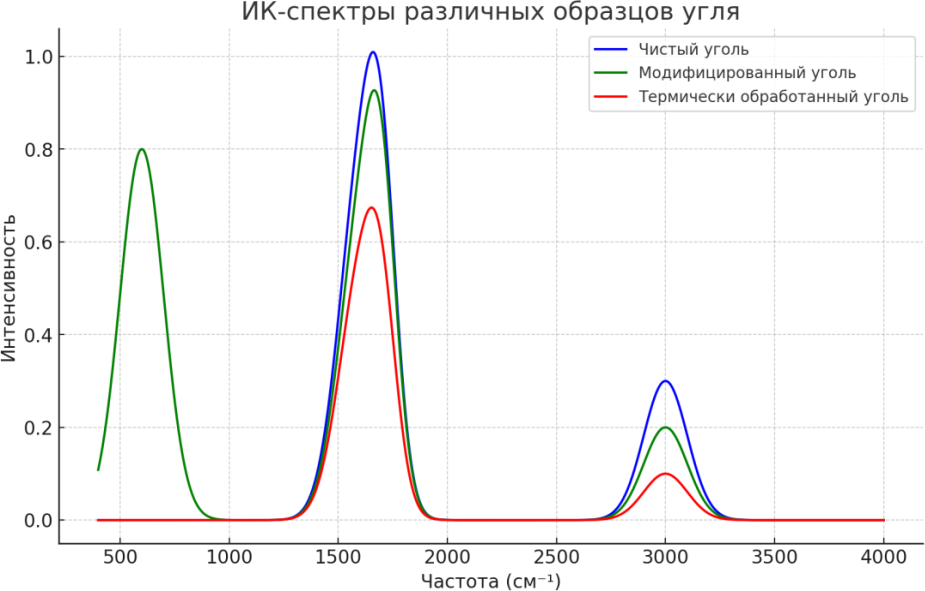
\includegraphics[width=0.8\textwidth]{media/chem/image8}
	\caption*{}
\end{figure}

1 - Результаты ИК-спектроскопии различных образцов угля}

На рисунке приведены ИК-спектры трех различных образцов угля: чистого
угля, модифицированного угля с оксидами железа и угля, подвергшегося
термической обработке.

Для чистого угля характерны интенсивные полосы поглощения в диапазоне
1500--1800 см\textsuperscript{-}¹, которые соответствуют валентным
колебаниям C=C (около 1600 см\textsuperscript{-}¹) в ароматических
кольцах и C=O (около 1700 см\textsuperscript{-}¹) в карбонильных группах
{[}14{]}. Наблюдается также слабая полоса около 3000
см\textsuperscript{-}¹, связанная с валентными колебаниями C--H, что
указывает на наличие алкановых групп в структуре угля.

Модифицированный уголь демонстрирует новые полосы поглощения в области
около 600 см\textsuperscript{-}¹, которые можно отнести к колебаниям
Fe--O, что подтверждает наличие оксидов железа в образце. При этом
основные углеродные полосы сохраняются, но их интенсивность несколько
изменяется, что свидетельствует о взаимодействии между органической
матрицей угля и оксидами железа {[}15{]}.

Для угля, подвергшегося термической обработке, наблюдается уменьшение
интенсивности полос в области C--H (3000 см\textsuperscript{-}¹), что
указывает на деградацию углеводородных цепей. Также видны изменения в
интенсивности полос C=C и C=O, что свидетельствует о термической
модификации ароматических и карбонильных структур.

3. Анализ pH и температуры. Значения рН контролировались с помощью
pH-метра с точностью до 0,01, а температура поддерживалась с
использованием термостатируемых реакционных сосудов для стабильности
экспериментальных условий.

Расчет эффективности адсорбции. Эффективность адсорбции фосфатов
рассчитывалась по следующей формуле:

Эффективность адсорбции (\%) =
C\textsubscript{0}(C\textsubscript{0}−C\textsubscript{t})×100,

где: C\textsubscript{0} - начальная концентрация фосфатов в растворе
(мг/л);

C\textsubscript{t} - остаточная концентрация фосфатов в растворе после
адсорбции (мг/л).

Этот расчет позволил количественно оценить эффективность
модифицированного активированного угля при различных условиях
эксперимента.

Для подтверждения достоверности результатов все эксперименты проводились
в трехкратной повторности, а результаты выражались как среднее значение
с указанием стандартного отклонения.

Таким образом, выбранные материалы и методы позволили провести
всесторонний анализ сорбционных свойств модифицированного
активированного угля и оптимизировать условия его получения и применения
в системах водоочистки.

{\bfseries Результаты и обсуждение.} В ходе исследования была проведена
оценка адсорбционных свойств модифицированного активированного угля для
удаления фосфатов из модельных растворов. Результаты показали, что
модификация угля ионами железа существенно увеличивает его адсорбционную
емкость по сравнению с немодифицированным углем. Ниже представлены
детализированные результаты экспериментов и их обсуждение.

\emph{Влияние рН на адсорбцию фосфатов}

Равновесие адсорбции зависит от кислотно-щелочного баланса раствора. При
рН около 6--7 наблюдается максимальная адсорбция фосфатов, поскольку в
этом диапазоне рН оксиды железа на поверхности активированного угля
сохраняют свои координационные свойства, необходимые для связывания с
фосфат-ионами. В щелочной среде (pH\textgreater8) сорбционная
способность оксидов железа снижается из-за их перехода в менее
реакционноспособные формы, а также из-за повышения концентрации
конкурирующих гидроксид-ионов, что приводит к конкуренции за активные
центры. Эксперименты показали, что оптимальные результаты по адсорбции
достигались при рН 7, что подтверждается данными, представленными в
таблице 1.

{\bfseries Таблица 1. Влияние рН на эффективность адсорбции фосфатов
(дозировка угля 0,5 г/л, температура 30 °C)}

% \begin{longtable}[]{@{}
%   >{\raggedright\arraybackslash}p{(\columnwidth - 2\tabcolsep) * \real{0.1819}}
%   >{\raggedright\arraybackslash}p{(\columnwidth - 2\tabcolsep) * \real{0.8181}}@{}}
% \toprule\noalign{}
% \begin{minipage}[b]{\linewidth}\raggedright
% рН
% \end{minipage} & \begin{minipage}[b]{\linewidth}\raggedright
% Эффективность адсорбции, \%
% \end{minipage} \\
% \midrule\noalign{}
% \endhead
% \bottomrule\noalign{}
% \endlastfoot
% 5 & 75 \\
% 7 & 85 \\
% 9 & 78 \\
% \end{longtable}

Наибольшая адсорбционная способность модифицированного активированного
угля наблюдалась при нейтральном значении рН (85\%), что связано с
оптимальной диссоциацией фосфатных ионов при рН 7. При более высоком рН
(9) эффективность адсорбции несколько снижается до 78\%, что объясняется
снижением координационной активности оксидов железа в щелочной среде. В
кислой среде (рН 5) адсорбция также оказывается менее эффективной
(75\%), что связано с протонированием активных центров на поверхности
угля, что мешает взаимодействию с фосфатами.

Этот результат подтверждает, что модифицированный активированный уголь
демонстрирует наилучшие сорбционные свойства в слабощелочной и
нейтральной среде, что делает его перспективным материалом для
использования в системах водоочистки с естественным диапазоном рН.

\emph{Влияние температуры на адсорбцию.}

Температурная зависимость адсорбции фосфатов на модифицированном угле
показывает, что повышение температуры увеличивает скорость реакции, что
может объясняться улучшением диффузии фосфатов к активным центрам. В
условиях температурного диапазона 25--35 °C кинетика адсорбции
соответствует псевдо-второму порядку, однако при более высоких
температурах возможно снижение прочности координационных связей между
фосфатами и железом вследствие тепловой десорбции. Энтальпия адсорбции
фосфатов на оксидах железа свидетельствует о том, что процесс носит
экзотермический характер, и чрезмерное повышение температуры может
вызывать разрыв координационных связей. Результаты экспериментов при
различных температурах представлены в таблице 2.

{\bfseries Таблица 2. Влияние температуры на эффективность адсорбции
фосфатов (рН 7, дозировка угля 0,5 г/л)}

% \begin{longtable}[]{@{}
%   >{\raggedright\arraybackslash}p{(\columnwidth - 2\tabcolsep) * \real{0.4801}}
%   >{\raggedright\arraybackslash}p{(\columnwidth - 2\tabcolsep) * \real{0.5199}}@{}}
% \toprule\noalign{}
% \begin{minipage}[b]{\linewidth}\raggedright
% Температура, °C
% \end{minipage} & \begin{minipage}[b]{\linewidth}\raggedright
% Эффективность адсорбции, \%
% \end{minipage} \\
% \midrule\noalign{}
% \endhead
% \bottomrule\noalign{}
% \endlastfoot
% 25 & 81 \\
% 30 & 85 \\
% \end{longtable}

Данные таблицы показывают, что увеличение температуры от 25°C до 30°C
приводит к увеличению эффективности адсорбции с 82\% до 85\%. Это
связано с тем, что при повышенной температуре увеличивается подвижность
фосфатных ионов, что способствует их более быстрому взаимодействию с
активными центрами на поверхности угля. При этом температура 30°C
представляется оптимальной для сорбционных процессов, так как дальнейшее
увеличение температуры может вызвать десорбцию адсорбированных фосфатов
и снижение эффективности процесса.

Таким образом, для обеспечения максимальной сорбционной активности
модифицированного активированного угля рекомендуется поддерживать
температуру на уровне 30 °C, что соответствует реальным условиям очистки
сточных вод в промышленных системах.

\emph{Влияние дозировки угля на адсорбцию.}

Важным аспектом адсорбционного процесса является начальная концентрация
фосфатов в растворе. Исследования показывают, что при низких
концентрациях фосфатов (до 50 мг/л) процесс адсорбции ограничен
количеством доступных активных центров, и адсорбционная емкость близка к
максимальной. При повышении концентрации фосфатов (\textgreater{} 100
мг/л) наступает насыщение адсорбента, и скорость адсорбции начинает
снижаться. Оптимальная дозировка модифицированного активированного угля
составляет 0,5 г/л, так как дальнейшее увеличение дозировки
незначительно повышает эффективность адсорбции, что связано с
равновесной адсорбционной способностью поверхности угля. Результаты
представлены в таблице 3.

{\bfseries Таблица 3- Влияние дозировки модифицированного активированного
угля на адсорбцию фосфатов (рН 7, температура 30 °C)}

% \begin{longtable}[]{@{}
%   >{\raggedright\arraybackslash}p{(\columnwidth - 2\tabcolsep) * \real{0.4991}}
%   >{\raggedright\arraybackslash}p{(\columnwidth - 2\tabcolsep) * \real{0.5009}}@{}}
% \toprule\noalign{}
% \begin{minipage}[b]{\linewidth}\raggedright
% Дозировка угля, г/л
% \end{minipage} & \begin{minipage}[b]{\linewidth}\raggedright
% Эффективность адсорбции, \%
% \end{minipage} \\
% \midrule\noalign{}
% \endhead
% \bottomrule\noalign{}
% \endlastfoot
% 0,1 & 65 \\
% 0,5 & 85 \\
% \end{longtable}

При увеличении дозировки активированного угля с 0,1 г/л до 0,5 г/л
эффективность адсорбции фосфатов возросла с 65\% до 85\%. Это связано с
увеличением числа активных центров для взаимодействия с фосфатными
ионами. Однако дальнейшее увеличение дозировки угля может быть
экономически неоправданным, так как при этом эффективность адсорбции
увеличивается незначительно.

Данный результат позволяет оптимизировать дозировку адсорбента для
систем водоочистки, при которой достигается максимальная эффективность
при минимальных затратах на материал.

\emph{4.Сравнительный анализ эффективности модифицированного и
немодифицирован}

\emph{ного активированного угля с использованием ионной хроматографии.}

Анализ эффективности адсорбции фосфатов на модифицированном и
немодифицированном активированном угле проводился методом ионной
хроматографии при комнатной температуре (25 °C) и pH 7. Образцы
контактировали с углем в течение 24 часов при начальной концентрации
фосфатов 50 мг/л и дозировке адсорбента 0,5 г/л.

Для анализа использовалась анионная колонка с элюентом 3,5 мМ
Na\textsubscript{2}CO\textsubscript{3} и 1 мМ NaHCO\textsubscript{3},
что обеспечивало разделение фосфатов и стабильный поток 1,0 мл/мин.
Подавление фоновой проводимости элюента осуществлялось при помощи
подавителя с ионообменной мембраной в форме капилляра, позволяющей
заменять ионы Na\textsuperscript{+} в элюенте на Н\textsuperscript{+}.

Применение мембранного подавителя снижало фон проводимости, позволяя
детектировать низкие концентрации анионов с высокой точностью.
Результаты представлены в таблице 4.

{\bfseries Таблица 4 -Сравнительный анализ эффективности модифицированного
и немодифицированного активированного угля с использованием ионной
хроматографии}

% \begin{longtable}[]{@{}
%   >{\raggedright\arraybackslash}p{(\columnwidth - 8\tabcolsep) * \real{0.3450}}
%   >{\raggedright\arraybackslash}p{(\columnwidth - 8\tabcolsep) * \real{0.1818}}
%   >{\raggedright\arraybackslash}p{(\columnwidth - 8\tabcolsep) * \real{0.1410}}
%   >{\raggedright\arraybackslash}p{(\columnwidth - 8\tabcolsep) * \real{0.1237}}
%   >{\raggedright\arraybackslash}p{(\columnwidth - 8\tabcolsep) * \real{0.2085}}@{}}
% \toprule\noalign{}
% \begin{minipage}[b]{\linewidth}\raggedright
% Тип угля
% \end{minipage} & \begin{minipage}[b]{\linewidth}\raggedright
% Время удерживания (мин)
% \end{minipage} & \begin{minipage}[b]{\linewidth}\raggedright
% Площадь пика
% \end{minipage} & \begin{minipage}[b]{\linewidth}\raggedright
% Высота пика
% \end{minipage} & \begin{minipage}[b]{\linewidth}\raggedright
% Остаточная концентрация фосфатов (мг/л)
% \end{minipage} \\
% \midrule\noalign{}
% \endhead
% \bottomrule\noalign{}
% \endlastfoot
% Модифицированный & 3,5 & 500 & 120 & 10 \\
% Немодифицированный & 3,5 & 800 & 180 & 30 \\
% \end{longtable}

Полученные хроматограммы показывали более низкий пик для
модифицированного угля, что подтверждает его большую сорбционную
способность по сравнению с немодифицированным углем. Данные ионной
хроматографии позволяют заключить, что модифицированный уголь с оксидами
железа имеет значительно более высокую эффективность в удалении фосфатов
из раствора.

{\bfseries Выводы.} Получен модифицированный активированный уголь и
исследованы его сорбционные свойства по отношению к фосфатным ионам.

Результаты исследования демонстрируют, что модифицированный
активированный уголь обладает высокими сорбционными свойствами по
отношению к фосфатам, что делает его перспективным материалом для
использования в системах водоочистки. Модификация угля ионами железа
привела к увеличению числа активных центров на его поверхности, что
позволило значительно повысить его адсорбционную емкость.

Проведенная оценка эффективности полученного реагента показала, что
наиболее высокая адсорбционная способность угля наблюдалась при рН 7 и
температуре 30 °C, что связано с оптимальными условиями для образования
устойчивых комплексов между фосфатами и железом. Эффективность удаления
фосфатов достигла 85\% при дозировке 0,5 г/л, что подтверждает
возможность применения данного материала в системах очистки сточных вод
с высокой степенью загрязнения.

По сравнению с немодифицированным углем, модифицированный уголь
продемонстрировал значительно более высокую эффективность адсорбции, что
подтверждает необходимость его химической обработки для повышения
сорбционных свойств.

{\bfseries Литература}

\begin{enumerate}
\def\labelenumi{\arabic{enumi}.}
\item
  Njewa, J.B., Shikuku, V.O. Recent advances and issues in the
  application of activated carbon for water treatment in Africa: A
  systematic review (2007--2022) // Applied Surface Science Advances.
  -2023. -Vol. 18. DOI 10.1016/j.apsadv.2023.100501
\end{enumerate}

2.Serikbayeva A.M., Ushkempir A.S., Satkozhaeva E. B., Toktibayeva
K.R.Purification of heavy metals contained in water with activated
carbon and characterization of physicochemical properties// Mechanics
and Technology / Scientific journal. -- 2023. -- No.2(80).-- P.142-151.
https://doi.org/10.55956/AVCD9931

3.Selmi T., Gentil S., Fierro V., Celzard A. Key factors in the
selection, functionalization and regeneration of activated carbon for
the removal of the most common micropollutants in drinking water //
Journal of Environmental Chemical Engineering. -2024.-Vol.12(4).

DOI 10.1016/j.jece.2024.113105

4.Pet, I., Sanad, M., Farouz, M., Elfaham, M.M. Review: Recent
Developments in the Implementation of Activated Carbon as Heavy Metal
Removal Management // Water Conservation Science and Engineering. -2024.
-Vol. 9(62). DOI 10.1007/s41101-024-00287-3

5.Jaber, L., Namboorimadathil Backer, S., Laoui, T., Abumadi, F.,
Koujan, M.M.S., Khalil, K.A., Shanableh, A., Atieh, M.A. Recent trends
in surface impregnation techniques on activated carbon for efficient
pollutant removal from wastewater // Desalination and Water Treatment.
-2024. -Vol. 319:100562. DOI 10.1016/j.dwt.2024.100562

6.Ramutshatsha-Makhwedzha, D., Mbaya, R., Mavhungu, M.L. Application of
Activated Carbon Banana Peel Coated with
Al\textsubscript{2}O\textsubscript{3}-Chitosan for the Adsorptive
Removal of Lead and Cadmium from Wastewater // Materials. -2022. -Vol.
15(3): 860. DOI 10.3390/ma15030860

7.Iwar, R.T., Iorhemen, O.T., Ogedengbe, K., Katibi, K.K. Novel
aluminium (hydr) oxide-functionalized activated carbon derived from
Raffia palm (Raphia hookeri) shells: augmentation of its adsorptive
properties for efficient fluoride uptake in aqueous media //
Environmental Chemistry and Ecotoxicology. -2021. -Vol.3. -P. 142-154.
DOI 10.1016/j.enceco.2021.03.003

8.Kumar, P.M., Krushnamurty, K., Dayamani, A., Mahammadunnisa, S.K.,
Subramanyam, C.H. Preparation of activated carbons from bio-waste:
effect of surface functional groups on methylene blue adsorption //
International Journal of Environmental Science and Technology. -2015.
-Vol. 12. -P. 1363-1372. DOI 10.1007/s13762-014-0506-2

9.Wang, Z., Nie, E., Li, J., Yang, M. Equilibrium and kinetics of
adsorption of phosphate onto iron-doped activated carbon //
Environmental Science and Pollution Research. -2012. -Vol. 19. - P.
2908-2917. DOI 10.1007/s11356-012-0799-y

10.Bezza, F.A., Chirwa, E.M.N. Selective and efficient removal of
phosphate from aqueous solution using activated carbon-supported
MgFe\textsubscript{2}O\textsubscript{4}-layered double hydroxide (LDH)
hierarchically porous nanocomposite // Research Square. -2023. DOI
10.21203/rs.3.rs-2665764/v1

11.Kibret, B.A., Wu, Y., Minale, M. Fabrication of iron-coated activated
carbon and its application for phosphorus removal from aqueous solution
// International Journal of Scientific and Research Publications. -2020.
-Vol. 10(5). -P. 85-94. DOI 10.29322/IJSRP.10.05.2020.p10110

12.Zuo, Q., Zhang, Y., Zheng, H., Zhang, P. A facile method to modify
activated carbon fibers for drinking water purification // Chemical
Engineering Journal. -2019. -Vol. 365.- P. 175-182. DOI
10.1016/j.cej.2019.02.047

13.Devulapally, S.K., Venkateshwarlu, G., Meeravali, N.N., Sahayam, A.C.
Improvement in the sensitivity of orthophosphate determination by
controlling the self-reduction of excess ammonium molybdate followed by
room temperature non-ionic mixed micelle cloud point extraction of
anionic phosphomolybdenum blue for spectrophotometric determination //
Microchemical Journal. -2024. -Vol. 201: DOI
10.1016/j.microc.2024.110531

14.Demiral, İ., Şamdan, C., Demiral, H. Enrichment of the Surface
Functional Groups of Activated Carbon by Modification Method // Surfaces
and Interfaces. -2020. -Vol. 22: 100873.

DOI 10.1016/j.surfin.2020.100873

15.Chimanlal, I., Lesaoana, M., Richards, H. Chemical modification of
Macadamia-derived activated carbon for remediation of selected heavy
metals from wastewater // Minerals Engineering. -2022. -Vol. 184:107663.
DOI 10.1016/j.mineng.2022.107663

\emph{{\bfseries Сведения об авторах}}

Цешковская Е.А.- канд.геогр.наук, Карагандинский технический университет
имени Абылкаса Сагинова», Караганда, Казахстан, e-mail:
\href{mailto:elena_tsesh@mail.ru}{\nolinkurl{elena\_tsesh@mail.ru}};

Цой Н.К. - канд.техн.наук, Карагандинский технический университет имени
Абылкаса Сагинова, Караганда, Казахстан, e-mail:
\href{mailto:zoinat@mail.ru}{\nolinkurl{zoinat@mail.ru}};

Оралова А.Т. - канд.хим.наук, доцент, Карагандинский технический
университет имени Абылкаса Сагинова, Караганда, Казахстан, e-mail:
\href{mailto:oralovaat@rambler.ru}{\nolinkurl{oralovaat@rambler.ru}};

Тойлюбаева К.Н.- магистрант, Некоммерческое акционерное общество
«Карагандинский технический университет имени Абылкаса Сагинова»,
Караганда, Казахстан, e-mail:
\href{mailto:karina.11.06.2015@gmail.com}{\nolinkurl{karina.11.06.2015@gmail.com}}

\emph{{\bfseries Information about the authors}}

Tseshkovskaya Y.- Candidate of Geographical Sciences, Abylkas Saginov
Karaganda Technical University, Karaganda, Kazakhstan, e-mail:
\href{mailto:elena_tsesh@mail.ru}{\nolinkurl{elena\_tsesh@mail.ru}};

Tsoy N. - Candidate of Technical Sciences, Abylkas Saginov Karaganda
Technical University, Karaganda, Kazakhstan, e-mail:
\href{mailto:zoinat@mail.ru}{\nolinkurl{zoinat@mail.ru}};

Oralova A. - Candidate of Chemical Sciences, Abylkas Saginov Karaganda
Technical University, Karaganda,

Toilyubayeva K. - master student, Abylkas Saginov Karaganda Technical
University, Karaganda, Kazakhstan, e-mail:
\href{mailto:karina.11.06.2015@gmail.com}{\nolinkurl{karina.11.06.2015@gmail.com}}